% Fig. 1 (Energy Systems): information arrival, equipment commitments and rental procurement. 
% Canvas 119 x 110 mm, coordinates in mm from
% the top-left corner, y downward. Black ink; categories by text and symbol (circle, triangle, square), not colour.
% Solid arrows: procurement and delivery; dashed: information; filled square: commitment; open square: availability.
\RequirePackage{fix-cm}
\documentclass[border=0pt]{standalone}
\usepackage[T1]{fontenc}
\usepackage{helvet}
\renewcommand{\familydefault}{\sfdefault}
\usepackage{amsmath}
\usepackage{sansmath}
\sansmath
\usepackage{tikz}
\usetikzlibrary{arrows.meta,calc,patterns,shapes.geometric}
\definecolor{ink}{HTML}{222222}
\definecolor{slate}{HTML}{666666}
\definecolor{neutF}{HTML}{F2F2F2}
\newcommand{\ttl}{\fontsize{9}{10.5}\selectfont\bfseries}
\newcommand{\lbl}{\fontsize{8}{9.5}\selectfont}
\newcommand{\sml}{\fontsize{7}{8.4}\selectfont}
\newcommand{\xq}[1]{\fpeval{34+5.75*(#1)}}
\begin{document}
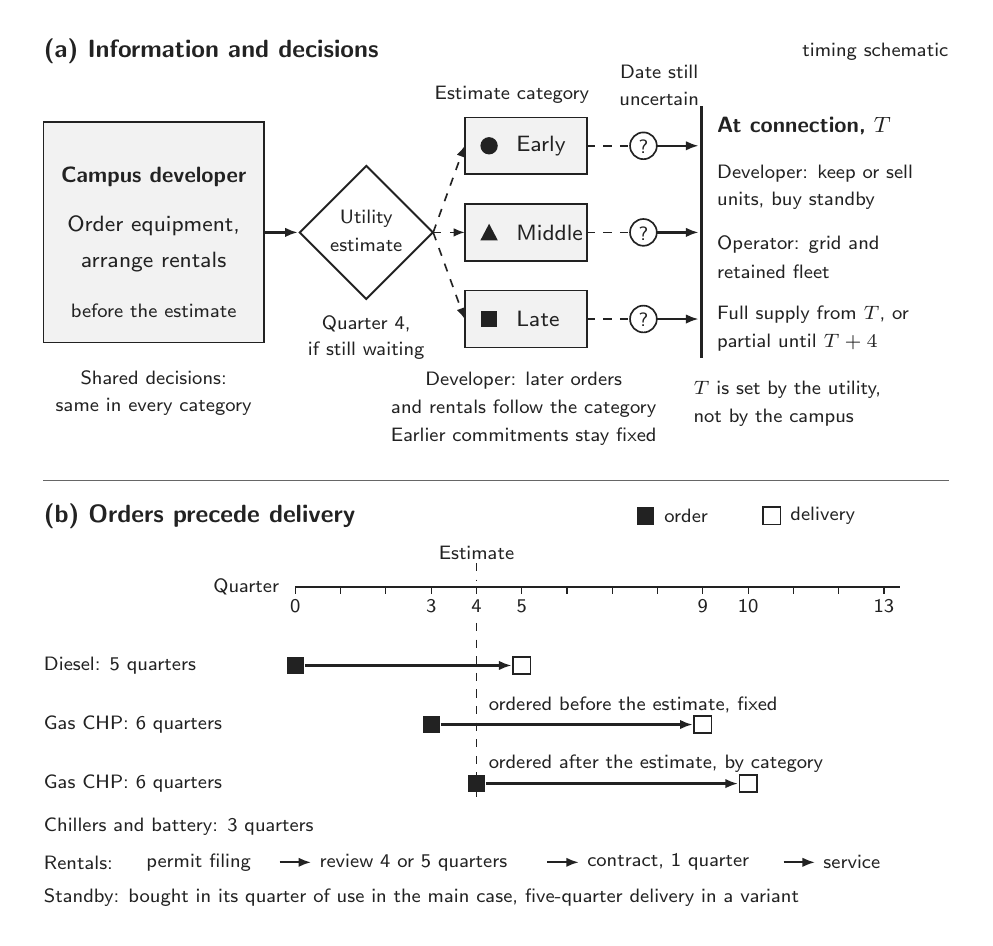
\begin{tikzpicture}[x=1mm, y=-1mm, every node/.style={text=ink, inner sep=0pt},
  proc/.style={draw=ink, line width=0.8pt, -{Latex[length=1.6mm,width=1.2mm]}},
  info/.style={draw=ink, line width=0.6pt, dashed, -{Latex[length=1.4mm,width=1.1mm]}},
  box/.style={draw=ink, fill=neutF, line width=0.6pt}]
\path (0,0) rectangle (119,113);

% ======================= (a) Information and decisions =======================
\node[anchor=west] at (2,3) {\ttl (a) Information and decisions};
\node[anchor=east] at (117,3) {\sml timing schematic};

% developer before the estimate
\draw[box] (2,12) rectangle (30,40);
\node[align=center] at (16,19) {\lbl\bfseries Campus developer};
\node[align=center] at (16,27.5) {\lbl Order equipment,\\[0.4mm]\lbl arrange rentals};
\node[align=center] at (16,36) {\sml before the estimate};
\node[align=center] at (16,44.5) {\sml Shared decisions:};
\node[align=center] at (16,48.2) {\sml same in every category};

% the estimate
\draw[proc] (30,26) -- (34.3,26);
\node[diamond, draw=ink, line width=0.7pt, fill=white, minimum width=17mm, minimum height=17mm, inner sep=0pt]
  (est) at (43,26) {};
\node[align=center] at (43,24.2) {\sml Utility};
\node[align=center] at (43,27.6) {\sml estimate};
\node[align=center] at (43,37.6) {\sml Quarter 4,};
\node[align=center] at (43,41.0) {\sml if still waiting};

% three categories
\node[align=center] at (61.5,8.5) {\sml Estimate category};
\foreach \y/\c in {15/Early, 26/Middle, 37/Late} {
  \draw[info] (51.5,26) -- (55.5,\y);
  \draw[box] (55.5,\y-3.6) rectangle (71,\y+3.6);
  \node[anchor=west] at (62,\y) {\lbl \c};
}
\fill[ink] (58.6,15) circle (1.1mm);
\fill[ink] (57.5,27) -- (59.7,27) -- (58.6,24.9) -- cycle;
\fill[ink] (57.6,36) rectangle (59.6,38);
\node[align=center] at (63,44.8) {\sml Developer: later orders};
\node[align=center] at (63,48.4) {\sml and rentals follow the category};
\node[align=center] at (63,52.0) {\sml Earlier commitments stay fixed};

% the actual date is still uncertain after each category
\node[align=center] at (80.2,5.6) {\sml Date still};
\node[align=center] at (80.2,9.0) {\sml uncertain};
\foreach \y in {15, 26, 37} {
  \draw[draw=ink, line width=0.6pt, dashed] (71,\y) -- (76.5,\y);
  \draw[draw=ink, line width=0.6pt, fill=white] (78.2,\y) circle (1.7mm);
  \node at (78.2,\y+0.15) {\sml ?};
  \draw[proc] (79.9,\y) -- (85.2,\y);
}
% connection event
\draw[draw=ink, line width=1.1pt] (85.6,10) -- (85.6,42);
\node[anchor=west] at (87.5,12.5) {\lbl\bfseries At connection, $T$};
\node[anchor=west] at (87.5,18.5) {\sml Developer: keep or sell};
\node[anchor=west] at (87.5,22.0) {\sml units, buy standby};
\node[anchor=west] at (87.5,27.5) {\sml Operator: grid and};
\node[anchor=west] at (87.5,31.0) {\sml retained fleet};
\node[anchor=west] at (87.5,36.5) {\sml Full supply from $T$, or};
\node[anchor=west] at (87.5,40.0) {\sml partial until $T+4$};
\node[anchor=west] at (84.5,46.0) {\sml $T$ is set by the utility,};
\node[anchor=west] at (84.5,49.5) {\sml not by the campus};

% ======================= (b) Orders precede delivery =======================
\draw[draw=slate, line width=0.4pt] (2,57.5) -- (117,57.5);
\node[anchor=west] at (2,62) {\ttl (b) Orders precede delivery};
\fill[ink] (77.4,60.9) rectangle (79.6,63.1);
\node[anchor=west] at (80.8,62) {\sml order};
\draw[draw=ink, line width=0.6pt, fill=white] (93.4,60.9) rectangle (95.6,63.1);
\node[anchor=west] at (96.8,62) {\sml delivery};

% quarter axis
\draw[draw=ink, line width=0.6pt] (\xq{0},71) -- (\xq{13}+2,71);
\foreach \q in {0,...,13} { \draw[draw=ink, line width=0.4pt] (\xq{\q},71) -- (\xq{\q},71.9); }
\foreach \q in {0,3,4,5,9,10,13} { \node[anchor=north] at (\xq{\q},72.6) {\sml \q}; }
\node[anchor=east] at (\xq{0}-2,71) {\sml Quarter};
\draw[draw=ink, line width=0.6pt, dashed] (\xq{4},68) -- (\xq{4},70.2);
\draw[draw=ink, line width=0.6pt, dashed] (\xq{4},75.6) -- (\xq{4},98);
\node[anchor=south] at (\xq{4},67.6) {\sml Estimate};

% order rows: filled square = order, open square = delivery; the note above each arrow says what the order is
\newcommand{\orderrow}[5]{%
  \node[anchor=west] at (2,#1) {\sml #4};
  \draw[proc] (\xq{#2}+1.2,#1) -- (\xq{#3}-1.3,#1);
  \fill[ink] (\xq{#2}-1.1,#1-1.1) rectangle (\xq{#2}+1.1,#1+1.1);
  \draw[draw=ink, line width=0.6pt, fill=white] (\xq{#3}-1.1,#1-1.1) rectangle (\xq{#3}+1.1,#1+1.1);
  \node[anchor=south west] at (\xq{4}+1.5,#1-1.4) {\sml #5};
}
\orderrow{81}{0}{5}{Diesel: 5 quarters}{}
\orderrow{88.5}{3}{9}{Gas CHP: 6 quarters}{ordered before the estimate, fixed}
\orderrow{96}{4}{10}{Gas CHP: 6 quarters}{ordered after the estimate, by category}
\node[anchor=west] at (2,101.5) {\sml Chillers and battery: 3 quarters};

% rental procurement strip
\node[anchor=west] at (2,106) {\sml Rentals:};
\node[anchor=west] at (15,106) {\sml permit filing};
\draw[proc] (32,106) -- (36,106);
\node[anchor=west] at (37,106) {\sml review 4 or 5 quarters};
\draw[proc] (66,106) -- (70,106);
\node[anchor=west] at (71,106) {\sml contract, 1 quarter};
\draw[proc] (96,106) -- (100,106);
\node[anchor=west] at (101,106) {\sml service};
\node[anchor=west] at (2,110.5) {\sml Standby: bought in its quarter of use in the main case, five-quarter delivery in a variant};
\end{tikzpicture}
\end{document}
